\section{simIrisComponentHeader.h File Reference}
\label{simIrisComponentHeader_8h}\index{simIrisComponentHeader.h@{simIrisComponentHeader.h}}
{\tt \#include $<$cstdlib$>$}\par
{\tt \#include $<$iostream$>$}\par
{\tt \#include $<$stdio.h$>$}\par
{\tt \#include $<$cassert$>$}\par
{\tt \#include \char`\"{}../kernel/simulator.h\char`\"{}}\par


Include dependency graph for simIrisComponentHeader.h:\nopagebreak
\begin{figure}[H]
\begin{center}
\leavevmode
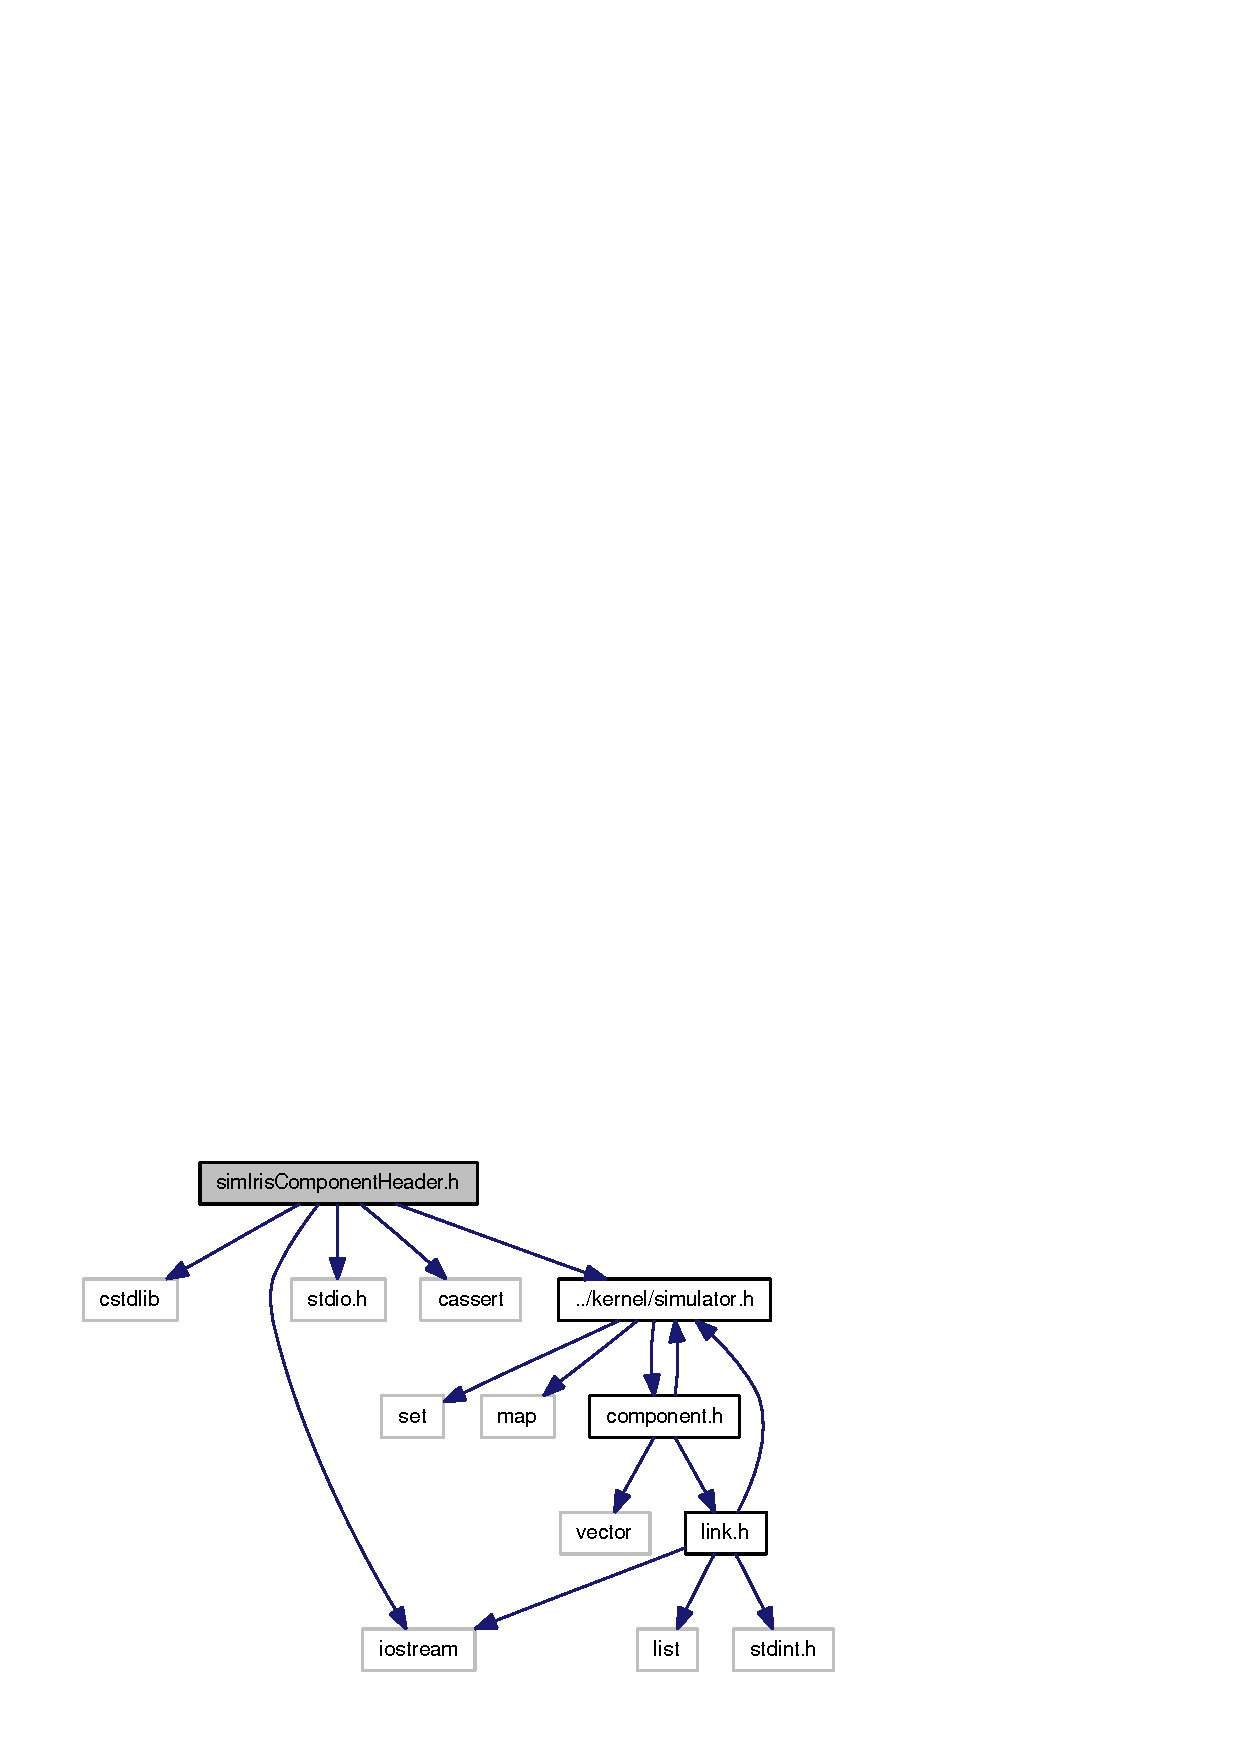
\includegraphics[width=202pt]{simIrisComponentHeader_8h__incl}
\end{center}
\end{figure}


This graph shows which files directly or indirectly include this file:\nopagebreak
\begin{figure}[H]
\begin{center}
\leavevmode
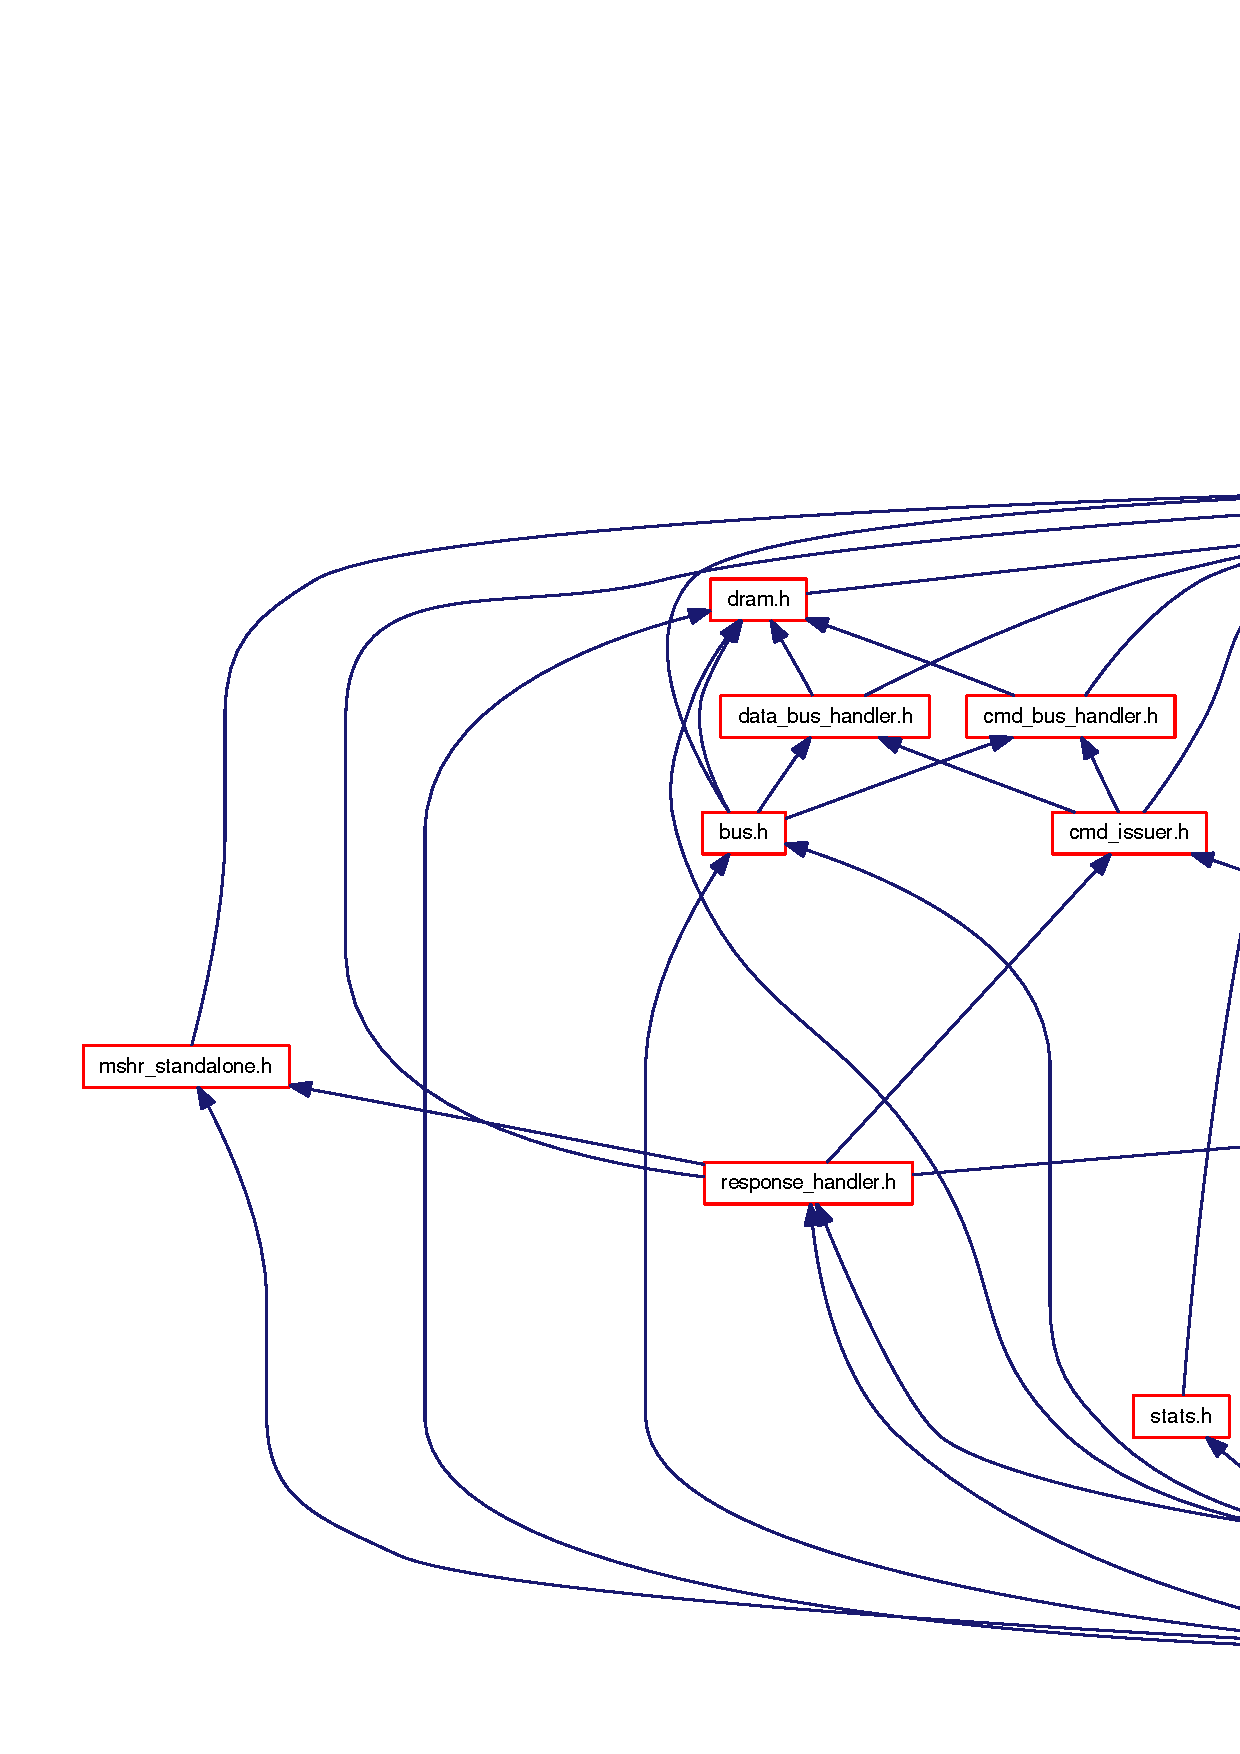
\includegraphics[width=420pt]{simIrisComponentHeader_8h__dep__incl}
\end{center}
\end{figure}
\subsection*{Defines}
\begin{CompactItemize}
\item 
\#define {\bf DEFAULT\_\-ADDRESS}~0
\item 
\#define {\bf DEFAULT\_\-CONVERT\_\-PACKET\_\-CYCLES}~1
\item 
\#define {\bf NO\_\-DATA}~true
\item 
\#define {\bf FLIT\_\-ID}~9800
\item 
\#define {\bf CREDIT\_\-ID}~9801
\item 
\#define {\bf LOC}~std::cout $<$$<$ \char`\"{}$\backslash$nTime:\char`\"{} $<$$<$ dec $<$$<$ Simulator::Now() $<$$<$\char`\"{} \char`\"{} $<$$<$ name $<$$<$ \char`\"{} \char`\"{} $<$$<$ address $<$$<$ \char`\"{} \char`\"{} $<$$<$ node\_\-ip $<$$<$ \char`\"{} \char`\"{};
\item 
\#define {\bf \_\-DBG}(fmt,...)~LOC printf(fmt,\_\-\_\-VA\_\-ARGS\_\-\_\-);
\item 
\#define {\bf \_\-DBG\_\-NOARG}(fmt)~LOC printf(fmt);
\end{CompactItemize}
\subsection*{Typedefs}
\begin{CompactItemize}
\item 
typedef unsigned long int {\bf uniqueId}
\item 
typedef unsigned long long int {\bf simTime}
\item 
typedef unsigned long long int {\bf ullint}
\item 
typedef unsigned int {\bf uint}
\end{CompactItemize}
\subsection*{Enumerations}
\begin{CompactItemize}
\item 
enum {\bf message\_\-class} \{ \par
{\bf INVALID\_\-PKT}, 
{\bf REQUEST\_\-PKT}, 
{\bf WRITE\_\-REQ}, 
{\bf RESPONSE\_\-PKT}, 
\par
{\bf ONE\_\-FLIT\_\-REQ}, 
{\bf CLUBBED\_\-PKT}, 
{\bf PRIORITY\_\-REQ}
 \}
\item 
enum {\bf virtual\_\-network} \{ {\bf VN0}, 
{\bf VN1}, 
{\bf VN2}
 \}
\end{CompactItemize}
\subsection*{Variables}
\begin{CompactItemize}
\item 
const unsigned int {\bf max\_\-network\_\-node\_\-bits} = 8
\item 
const unsigned int {\bf max\_\-transaction\_\-id\_\-bits} = 8
\item 
const unsigned int {\bf max\_\-tail\_\-length\_\-bits} = 8
\item 
const unsigned int {\bf max\_\-control\_\-bits} = 8
\item 
const unsigned int {\bf max\_\-pkt\_\-cnt\_\-bits} = 3
\item 
const unsigned int {\bf head\_\-and\_\-tail\_\-length} = 80
\end{CompactItemize}


\subsection{Define Documentation}
\index{simIrisComponentHeader.h@{simIrisComponentHeader.h}!\_\-DBG@{\_\-DBG}}
\index{\_\-DBG@{\_\-DBG}!simIrisComponentHeader.h@{simIrisComponentHeader.h}}
\subsubsection[{\_\-DBG}]{\setlength{\rightskip}{0pt plus 5cm}\#define \_\-DBG(fmt, \/   {\em ...})~LOC printf(fmt,\_\-\_\-VA\_\-ARGS\_\-\_\-);}\label{simIrisComponentHeader_8h_db8be0abb314b4cd0da20a9aa45a473e}




Definition at line 37 of file simIrisComponentHeader.h.

Referenced by GenericVcAllocator::clear\_\-winner(), GenericRouterVct::do\_\-switch\_\-allocation(), GenericRouterNoVcs::do\_\-switch\_\-allocation(), GenericRouterVct::do\_\-switch\_\-traversal(), GenericRouterVcs::do\_\-switch\_\-traversal(), GenericRouterNoVcs::do\_\-switch\_\-traversal(), GenericRouterAdaptive::do\_\-switch\_\-traversal(), GenericVcArbiter::empty(), GenericInterfaceVcs::handle\_\-link\_\-arrival(), GenericInterface::handle\_\-link\_\-arrival(), GenericRouterVct::handle\_\-link\_\-arrival\_\-event(), GenericRouterVcs::handle\_\-link\_\-arrival\_\-event(), GenericRouterNoVcs::handle\_\-link\_\-arrival\_\-event(), GenericLink::handle\_\-link\_\-arrival\_\-event(), GenericRouterAdaptive::handle\_\-link\_\-arrival\_\-event\_\-multiple\_\-flit\_\-in\_\-buffer(), GenericRouterAdaptive::handle\_\-link\_\-arrival\_\-event\_\-one\_\-msg\_\-per\_\-buffer(), NI::handle\_\-new\_\-packet\_\-event(), GenericTPGVcs::handle\_\-new\_\-packet\_\-event(), GenericTPG::handle\_\-new\_\-packet\_\-event(), GenericRPG::handle\_\-new\_\-packet\_\-event(), GenericInterfaceVcs::handle\_\-new\_\-packet\_\-event(), GenericInterface::handle\_\-new\_\-packet\_\-event(), GenericTPGVcs::handle\_\-out\_\-pull\_\-event(), GenericTPG::handle\_\-out\_\-pull\_\-event(), GenericSink::handle\_\-outpull\_\-event(), NI::handle\_\-ready\_\-event(), GenericTPGVcs::handle\_\-ready\_\-event(), GenericInterfaceVcs::handle\_\-ready\_\-event(), GenericInterface::handle\_\-ready\_\-event(), GenericRouterVct::handle\_\-tick\_\-event(), GenericRouterNoVcs::handle\_\-tick\_\-event(), GenericRouterAdaptive::handle\_\-tick\_\-event(), GenericInterfaceVcs::handle\_\-tick\_\-event(), GenericInterface::handle\_\-tick\_\-event(), GenericVcArbiter::is\_\-requested(), GenericVcArbiter::pick\_\-winner(), GenericRouterVct::process\_\-event(), GenericRouterVcs::process\_\-event(), GenericRouterNoVcs::process\_\-event(), GenericRouterAdaptive::process\_\-event(), GenericVcArbiter::pull\_\-winner(), GenericRC::push(), GenericRC::route\_\-negative\_\-first(), GenericRC::route\_\-north\_\-last(), GenericRC::route\_\-north\_\-last\_\-non\_\-minimal(), GenericRC::route\_\-odd\_\-even(), GenericRC::route\_\-west\_\-first(), GenericRC::route\_\-x\_\-y(), GenericRouterVct::send\_\-credit\_\-back(), GenericRouterNoVcs::send\_\-credit\_\-back(), and GenericRouterAdaptive::send\_\-credit\_\-back().\index{simIrisComponentHeader.h@{simIrisComponentHeader.h}!\_\-DBG\_\-NOARG@{\_\-DBG\_\-NOARG}}
\index{\_\-DBG\_\-NOARG@{\_\-DBG\_\-NOARG}!simIrisComponentHeader.h@{simIrisComponentHeader.h}}
\subsubsection[{\_\-DBG\_\-NOARG}]{\setlength{\rightskip}{0pt plus 5cm}\#define \_\-DBG\_\-NOARG(fmt)~LOC printf(fmt);}\label{simIrisComponentHeader_8h_34e0f121e3b717b1a15c6f90dae9f5d5}




Definition at line 38 of file simIrisComponentHeader.h.

Referenced by PToPSwitchArbiter::do\_\-fcfs\_\-arbitration(), PToPSwitchArbiter::do\_\-priority\_\-round\_\-robin\_\-arbitration(), PToPSwitchArbiterVcs::do\_\-round\_\-robin\_\-arbitration(), PToPSwitchArbiter::do\_\-round\_\-robin\_\-arbitration(), GenericRouterVct::do\_\-switch\_\-traversal(), GenericRouterNoVcs::do\_\-switch\_\-traversal(), GenericRouterVcs::handle\_\-detect\_\-deadlock\_\-event(), GenericRPG::handle\_\-ready\_\-event(), GenericFlatMc::handle\_\-ready\_\-event(), GenericRouterVct::handle\_\-tick\_\-event(), GenericRouterNoVcs::handle\_\-tick\_\-event(), and GenericRC::push().\index{simIrisComponentHeader.h@{simIrisComponentHeader.h}!CREDIT\_\-ID@{CREDIT\_\-ID}}
\index{CREDIT\_\-ID@{CREDIT\_\-ID}!simIrisComponentHeader.h@{simIrisComponentHeader.h}}
\subsubsection[{CREDIT\_\-ID}]{\setlength{\rightskip}{0pt plus 5cm}\#define CREDIT\_\-ID~9801}\label{simIrisComponentHeader_8h_2d879516eff32a88299e25eb5a377fee}




Definition at line 27 of file simIrisComponentHeader.h.

Referenced by GenericInterfaceVcs::handle\_\-link\_\-arrival(), GenericInterface::handle\_\-link\_\-arrival(), GenericRouterVct::handle\_\-link\_\-arrival\_\-event(), GenericRouterVcs::handle\_\-link\_\-arrival\_\-event(), GenericRouterNoVcs::handle\_\-link\_\-arrival\_\-event(), GenericRouterAdaptive::handle\_\-link\_\-arrival\_\-event\_\-multiple\_\-flit\_\-in\_\-buffer(), GenericRouterAdaptive::handle\_\-link\_\-arrival\_\-event\_\-one\_\-msg\_\-per\_\-buffer(), GenericInterfaceVcs::handle\_\-tick\_\-event(), GenericInterface::handle\_\-tick\_\-event(), GenericRouterVct::send\_\-credit\_\-back(), GenericRouterVcs::send\_\-credit\_\-back(), GenericRouterNoVcs::send\_\-credit\_\-back(), and GenericRouterAdaptive::send\_\-credit\_\-back().\index{simIrisComponentHeader.h@{simIrisComponentHeader.h}!DEFAULT\_\-ADDRESS@{DEFAULT\_\-ADDRESS}}
\index{DEFAULT\_\-ADDRESS@{DEFAULT\_\-ADDRESS}!simIrisComponentHeader.h@{simIrisComponentHeader.h}}
\subsubsection[{DEFAULT\_\-ADDRESS}]{\setlength{\rightskip}{0pt plus 5cm}\#define DEFAULT\_\-ADDRESS~0}\label{simIrisComponentHeader_8h_838ee749ec1dfd8d73187bb32e9ec427}




Definition at line 23 of file simIrisComponentHeader.h.\index{simIrisComponentHeader.h@{simIrisComponentHeader.h}!DEFAULT\_\-CONVERT\_\-PACKET\_\-CYCLES@{DEFAULT\_\-CONVERT\_\-PACKET\_\-CYCLES}}
\index{DEFAULT\_\-CONVERT\_\-PACKET\_\-CYCLES@{DEFAULT\_\-CONVERT\_\-PACKET\_\-CYCLES}!simIrisComponentHeader.h@{simIrisComponentHeader.h}}
\subsubsection[{DEFAULT\_\-CONVERT\_\-PACKET\_\-CYCLES}]{\setlength{\rightskip}{0pt plus 5cm}\#define DEFAULT\_\-CONVERT\_\-PACKET\_\-CYCLES~1}\label{simIrisComponentHeader_8h_4cd25c48b8874affbec9785d9d4ba055}




Definition at line 24 of file simIrisComponentHeader.h.\index{simIrisComponentHeader.h@{simIrisComponentHeader.h}!FLIT\_\-ID@{FLIT\_\-ID}}
\index{FLIT\_\-ID@{FLIT\_\-ID}!simIrisComponentHeader.h@{simIrisComponentHeader.h}}
\subsubsection[{FLIT\_\-ID}]{\setlength{\rightskip}{0pt plus 5cm}\#define FLIT\_\-ID~9800}\label{simIrisComponentHeader_8h_4c17fe87d84664c123df538e6be7fa5c}




Definition at line 26 of file simIrisComponentHeader.h.

Referenced by GenericRouterVct::do\_\-switch\_\-traversal(), GenericRouterVcs::do\_\-switch\_\-traversal(), GenericRouterNoVcs::do\_\-switch\_\-traversal(), GenericRouterAdaptive::do\_\-switch\_\-traversal(), GenericInterfaceVcs::handle\_\-link\_\-arrival(), GenericInterface::handle\_\-link\_\-arrival(), GenericRouterVct::handle\_\-link\_\-arrival\_\-event(), GenericRouterVcs::handle\_\-link\_\-arrival\_\-event(), GenericRouterNoVcs::handle\_\-link\_\-arrival\_\-event(), GenericRouterAdaptive::handle\_\-link\_\-arrival\_\-event\_\-multiple\_\-flit\_\-in\_\-buffer(), GenericRouterAdaptive::handle\_\-link\_\-arrival\_\-event\_\-one\_\-msg\_\-per\_\-buffer(), GenericInterfaceVcs::handle\_\-tick\_\-event(), and GenericInterface::handle\_\-tick\_\-event().\index{simIrisComponentHeader.h@{simIrisComponentHeader.h}!LOC@{LOC}}
\index{LOC@{LOC}!simIrisComponentHeader.h@{simIrisComponentHeader.h}}
\subsubsection[{LOC}]{\setlength{\rightskip}{0pt plus 5cm}\#define LOC~std::cout $<$$<$ \char`\"{}$\backslash$nTime:\char`\"{} $<$$<$ dec $<$$<$ Simulator::Now() $<$$<$\char`\"{} \char`\"{} $<$$<$ name $<$$<$ \char`\"{} \char`\"{} $<$$<$ address $<$$<$ \char`\"{} \char`\"{} $<$$<$ node\_\-ip $<$$<$ \char`\"{} \char`\"{};}\label{simIrisComponentHeader_8h_0fee446a4a4ef6536664bc1ff47ff694}




Definition at line 36 of file simIrisComponentHeader.h.\index{simIrisComponentHeader.h@{simIrisComponentHeader.h}!NO\_\-DATA@{NO\_\-DATA}}
\index{NO\_\-DATA@{NO\_\-DATA}!simIrisComponentHeader.h@{simIrisComponentHeader.h}}
\subsubsection[{NO\_\-DATA}]{\setlength{\rightskip}{0pt plus 5cm}\#define NO\_\-DATA~true}\label{simIrisComponentHeader_8h_68de9030c39965958f08402f7d452ad9}




Definition at line 25 of file simIrisComponentHeader.h.

\subsection{Typedef Documentation}
\index{simIrisComponentHeader.h@{simIrisComponentHeader.h}!simTime@{simTime}}
\index{simTime@{simTime}!simIrisComponentHeader.h@{simIrisComponentHeader.h}}
\subsubsection[{simTime}]{\setlength{\rightskip}{0pt plus 5cm}typedef unsigned long long int {\bf simTime}}\label{simIrisComponentHeader_8h_d88faca783e7aa496cda721d9029a2e3}




Definition at line 44 of file simIrisComponentHeader.h.\index{simIrisComponentHeader.h@{simIrisComponentHeader.h}!uint@{uint}}
\index{uint@{uint}!simIrisComponentHeader.h@{simIrisComponentHeader.h}}
\subsubsection[{uint}]{\setlength{\rightskip}{0pt plus 5cm}typedef unsigned int {\bf uint}}\label{simIrisComponentHeader_8h_91ad9478d81a7aaf2593e8d9c3d06a14}




Definition at line 46 of file simIrisComponentHeader.h.\index{simIrisComponentHeader.h@{simIrisComponentHeader.h}!ullint@{ullint}}
\index{ullint@{ullint}!simIrisComponentHeader.h@{simIrisComponentHeader.h}}
\subsubsection[{ullint}]{\setlength{\rightskip}{0pt plus 5cm}typedef unsigned long long int {\bf ullint}}\label{simIrisComponentHeader_8h_b03b0cc5e09b0e1f1ca05c2502cb93f4}




Definition at line 45 of file simIrisComponentHeader.h.\index{simIrisComponentHeader.h@{simIrisComponentHeader.h}!uniqueId@{uniqueId}}
\index{uniqueId@{uniqueId}!simIrisComponentHeader.h@{simIrisComponentHeader.h}}
\subsubsection[{uniqueId}]{\setlength{\rightskip}{0pt plus 5cm}typedef unsigned long int {\bf uniqueId}}\label{simIrisComponentHeader_8h_880960a57c549f69d77cf01237366978}




Definition at line 43 of file simIrisComponentHeader.h.

\subsection{Enumeration Type Documentation}
\index{simIrisComponentHeader.h@{simIrisComponentHeader.h}!message\_\-class@{message\_\-class}}
\index{message\_\-class@{message\_\-class}!simIrisComponentHeader.h@{simIrisComponentHeader.h}}
\subsubsection[{message\_\-class}]{\setlength{\rightskip}{0pt plus 5cm}enum {\bf message\_\-class}}\label{simIrisComponentHeader_8h_155eefa40b3e6db305cb151f7bb6bef4}


\begin{Desc}
\item[Enumerator: ]\par
\begin{description}
\index{INVALID\_\-PKT@{INVALID\_\-PKT}!simIrisComponentHeader.h@{simIrisComponentHeader.h}}\index{simIrisComponentHeader.h@{simIrisComponentHeader.h}!INVALID\_\-PKT@{INVALID\_\-PKT}}\item[{\em 
INVALID\_\-PKT\label{simIrisComponentHeader_8h_155eefa40b3e6db305cb151f7bb6bef4e7fe9d12722f3ee42b17fc4c9c04faba}
}]\index{REQUEST\_\-PKT@{REQUEST\_\-PKT}!simIrisComponentHeader.h@{simIrisComponentHeader.h}}\index{simIrisComponentHeader.h@{simIrisComponentHeader.h}!REQUEST\_\-PKT@{REQUEST\_\-PKT}}\item[{\em 
REQUEST\_\-PKT\label{simIrisComponentHeader_8h_155eefa40b3e6db305cb151f7bb6bef4d3e842c7a5ceb4faa20853be6b41b8db}
}]\index{WRITE\_\-REQ@{WRITE\_\-REQ}!simIrisComponentHeader.h@{simIrisComponentHeader.h}}\index{simIrisComponentHeader.h@{simIrisComponentHeader.h}!WRITE\_\-REQ@{WRITE\_\-REQ}}\item[{\em 
WRITE\_\-REQ\label{simIrisComponentHeader_8h_155eefa40b3e6db305cb151f7bb6bef44b69f4b601ec9ab61dde94aadd61f5f8}
}]\index{RESPONSE\_\-PKT@{RESPONSE\_\-PKT}!simIrisComponentHeader.h@{simIrisComponentHeader.h}}\index{simIrisComponentHeader.h@{simIrisComponentHeader.h}!RESPONSE\_\-PKT@{RESPONSE\_\-PKT}}\item[{\em 
RESPONSE\_\-PKT\label{simIrisComponentHeader_8h_155eefa40b3e6db305cb151f7bb6bef4294528b7f87e4eee5d8f8ce252480ee1}
}]\index{ONE\_\-FLIT\_\-REQ@{ONE\_\-FLIT\_\-REQ}!simIrisComponentHeader.h@{simIrisComponentHeader.h}}\index{simIrisComponentHeader.h@{simIrisComponentHeader.h}!ONE\_\-FLIT\_\-REQ@{ONE\_\-FLIT\_\-REQ}}\item[{\em 
ONE\_\-FLIT\_\-REQ\label{simIrisComponentHeader_8h_155eefa40b3e6db305cb151f7bb6bef462d2a16eab393943696ee3dce69c15d6}
}]\index{CLUBBED\_\-PKT@{CLUBBED\_\-PKT}!simIrisComponentHeader.h@{simIrisComponentHeader.h}}\index{simIrisComponentHeader.h@{simIrisComponentHeader.h}!CLUBBED\_\-PKT@{CLUBBED\_\-PKT}}\item[{\em 
CLUBBED\_\-PKT\label{simIrisComponentHeader_8h_155eefa40b3e6db305cb151f7bb6bef4155897a00b1a5373c29d5a196a318184}
}]\index{PRIORITY\_\-REQ@{PRIORITY\_\-REQ}!simIrisComponentHeader.h@{simIrisComponentHeader.h}}\index{simIrisComponentHeader.h@{simIrisComponentHeader.h}!PRIORITY\_\-REQ@{PRIORITY\_\-REQ}}\item[{\em 
PRIORITY\_\-REQ\label{simIrisComponentHeader_8h_155eefa40b3e6db305cb151f7bb6bef40ac409ee0059f317bf64a33cd711732f}
}]\end{description}
\end{Desc}



Definition at line 47 of file simIrisComponentHeader.h.\index{simIrisComponentHeader.h@{simIrisComponentHeader.h}!virtual\_\-network@{virtual\_\-network}}
\index{virtual\_\-network@{virtual\_\-network}!simIrisComponentHeader.h@{simIrisComponentHeader.h}}
\subsubsection[{virtual\_\-network}]{\setlength{\rightskip}{0pt plus 5cm}enum {\bf virtual\_\-network}}\label{simIrisComponentHeader_8h_2f11671ee174f5c324e71f348aef6e96}


\begin{Desc}
\item[Enumerator: ]\par
\begin{description}
\index{VN0@{VN0}!simIrisComponentHeader.h@{simIrisComponentHeader.h}}\index{simIrisComponentHeader.h@{simIrisComponentHeader.h}!VN0@{VN0}}\item[{\em 
VN0\label{simIrisComponentHeader_8h_2f11671ee174f5c324e71f348aef6e965a2c02cda17c1d1485f54eb64a089c7e}
}]\index{VN1@{VN1}!simIrisComponentHeader.h@{simIrisComponentHeader.h}}\index{simIrisComponentHeader.h@{simIrisComponentHeader.h}!VN1@{VN1}}\item[{\em 
VN1\label{simIrisComponentHeader_8h_2f11671ee174f5c324e71f348aef6e96fd42715ed367a6ef720bfa3be9036a8b}
}]\index{VN2@{VN2}!simIrisComponentHeader.h@{simIrisComponentHeader.h}}\index{simIrisComponentHeader.h@{simIrisComponentHeader.h}!VN2@{VN2}}\item[{\em 
VN2\label{simIrisComponentHeader_8h_2f11671ee174f5c324e71f348aef6e966135954823d9c9f5666429f69bc17fe3}
}]\end{description}
\end{Desc}



Definition at line 58 of file simIrisComponentHeader.h.

\subsection{Variable Documentation}
\index{simIrisComponentHeader.h@{simIrisComponentHeader.h}!head\_\-and\_\-tail\_\-length@{head\_\-and\_\-tail\_\-length}}
\index{head\_\-and\_\-tail\_\-length@{head\_\-and\_\-tail\_\-length}!simIrisComponentHeader.h@{simIrisComponentHeader.h}}
\subsubsection[{head\_\-and\_\-tail\_\-length}]{\setlength{\rightskip}{0pt plus 5cm}const unsigned int {\bf head\_\-and\_\-tail\_\-length} = 80}\label{simIrisComponentHeader_8h_8dbcbbf46fb808cab854d20ce33645d5}




Definition at line 56 of file simIrisComponentHeader.h.\index{simIrisComponentHeader.h@{simIrisComponentHeader.h}!max\_\-control\_\-bits@{max\_\-control\_\-bits}}
\index{max\_\-control\_\-bits@{max\_\-control\_\-bits}!simIrisComponentHeader.h@{simIrisComponentHeader.h}}
\subsubsection[{max\_\-control\_\-bits}]{\setlength{\rightskip}{0pt plus 5cm}const unsigned int {\bf max\_\-control\_\-bits} = 8}\label{simIrisComponentHeader_8h_3c2da81fd84ab0358092e3b47aac3b3c}




Definition at line 52 of file simIrisComponentHeader.h.\index{simIrisComponentHeader.h@{simIrisComponentHeader.h}!max\_\-network\_\-node\_\-bits@{max\_\-network\_\-node\_\-bits}}
\index{max\_\-network\_\-node\_\-bits@{max\_\-network\_\-node\_\-bits}!simIrisComponentHeader.h@{simIrisComponentHeader.h}}
\subsubsection[{max\_\-network\_\-node\_\-bits}]{\setlength{\rightskip}{0pt plus 5cm}const unsigned int {\bf max\_\-network\_\-node\_\-bits} = 8}\label{simIrisComponentHeader_8h_a11688d7b68d9e3b60784e388b3a94c8}




Definition at line 49 of file simIrisComponentHeader.h.

Referenced by HeadFlit::populate\_\-head\_\-flit().\index{simIrisComponentHeader.h@{simIrisComponentHeader.h}!max\_\-pkt\_\-cnt\_\-bits@{max\_\-pkt\_\-cnt\_\-bits}}
\index{max\_\-pkt\_\-cnt\_\-bits@{max\_\-pkt\_\-cnt\_\-bits}!simIrisComponentHeader.h@{simIrisComponentHeader.h}}
\subsubsection[{max\_\-pkt\_\-cnt\_\-bits}]{\setlength{\rightskip}{0pt plus 5cm}const unsigned int {\bf max\_\-pkt\_\-cnt\_\-bits} = 3}\label{simIrisComponentHeader_8h_3c6f8fc634796e799dfe8c3d848abd40}




Definition at line 55 of file simIrisComponentHeader.h.

Referenced by HeadFlit::populate\_\-head\_\-flit().\index{simIrisComponentHeader.h@{simIrisComponentHeader.h}!max\_\-tail\_\-length\_\-bits@{max\_\-tail\_\-length\_\-bits}}
\index{max\_\-tail\_\-length\_\-bits@{max\_\-tail\_\-length\_\-bits}!simIrisComponentHeader.h@{simIrisComponentHeader.h}}
\subsubsection[{max\_\-tail\_\-length\_\-bits}]{\setlength{\rightskip}{0pt plus 5cm}const unsigned int {\bf max\_\-tail\_\-length\_\-bits} = 8}\label{simIrisComponentHeader_8h_5865e4b460e585b9a53f2dfa6a5839ae}




Definition at line 51 of file simIrisComponentHeader.h.

Referenced by TailFlit::populate\_\-tail\_\-flit().\index{simIrisComponentHeader.h@{simIrisComponentHeader.h}!max\_\-transaction\_\-id\_\-bits@{max\_\-transaction\_\-id\_\-bits}}
\index{max\_\-transaction\_\-id\_\-bits@{max\_\-transaction\_\-id\_\-bits}!simIrisComponentHeader.h@{simIrisComponentHeader.h}}
\subsubsection[{max\_\-transaction\_\-id\_\-bits}]{\setlength{\rightskip}{0pt plus 5cm}const unsigned int {\bf max\_\-transaction\_\-id\_\-bits} = 8}\label{simIrisComponentHeader_8h_df297dfc5bd1387de6bec325bfa30f23}




Definition at line 50 of file simIrisComponentHeader.h.

Referenced by HeadFlit::populate\_\-head\_\-flit().